\documentclass[xcolor=dvipsnames,beamer]{beamer} %handout,notes=show

\usepackage{textcomp}
\usepackage[utf8]{inputenc}
% \usepackage{default}
\usepackage{graphicx}
%  \usepackage[pdftex]{hyperref}
\usepackage{url}
\usepackage{amsmath}

% frames have to be fragile
\newif\ifnotes
% \notestrue

%\notestrue


\ifnotes
%\setbeamertemplate{note page}[plain]
\setbeamertemplate{note page}[compress]
\setbeamerfont{note page}{size=\large}
\setbeameroption{show only notes}
%\setbeameroption{show notes}
\usepackage{pgfpages}
\pgfpagesuselayout{2 on 1}[a4paper,border shrink=5mm]%
\else
%\setbeameroption{hide notes}
\fi
%\notesfalse



% nastaveni TypeWriter
%\usepackage{courier}
%\usepackage{lmodern}
%\renewcommand*\ttdefault{txtt}
\DeclareFontShape{OT1}{cmtt}{bx}{n}{<5><6><7><8><9><10><10.95><12><14.4><17.28><20.74><24.88>cmttb10}{}


% \usepackage{verbatim}
\usepackage[absolute,overlay]{textpos}

\usepackage{listings}
% \usepackage{courier}
\definecolor{grey}{RGB}{70,70,70}
\definecolor{green}{RGB}{0,255,0}
\definecolor{red}{RGB}{202,53,53}
\definecolor{lightGrey}{RGB}{250,250,250}
\definecolor{darkGrey}{RGB}{50,50,50}


\usepackage{color}
\definecolor{lightgray}{rgb}{.9,.9,.9}
\definecolor{darkgray}{rgb}{.4,.4,.4}
\definecolor{purple}{rgb}{0.65, 0.12, 0.82}


% \usetheme{Warsaw}
% \usetheme{Madrid}
\usetheme{Szeged}
% \useoutertheme{infolines}
\usecolortheme[named=MidnightBlue]{structure}
% \usecolortheme[named=PineGreen]{structure}
% \setbeamertemplate{navigation symbols}{}




\title[Flood \& Drought Crop Risk]
{Flood and Drought Crop Risk}
%\subtitle{SVO\v{C}}
%\pdforstring{}{}
\author[Yann Chemin]
{Yann Chemin}

\institute[IWMI]
{International Water Management Institute
\vspace{20pt}
% 
\includegraphics[width=1cm]{iwmi}
}
\date{June 12, 2013}


%\AtBeginSection[]{\begin{frame}\frametitle{Obsah}%
%\tableofcontents[currentsection ]\end{frame}}
%\AtBeginSubsection[]
%{
%  \begin{frame}<beamer>
%  \frametitle{Obsah}
%  \tableofcontents[currentsection,currentsubsection]
%  \end{frame}
%}

\setbeamercovered{transparent}

\hypersetup{%
	pdfauthor={Yann Chemin},%
	pdfsubject={Presentation},%
    pdfkeywords={flood, drought, crops, IWMI}
}

\usepackage{listings}
\lstdefinestyle{C++}{%
  % language
  language=C++, % [ANSI]C++, GNU, ISO, Visual
  basicstyle=\ttfamily\small,
  commentstyle=\itshape,
  keywordstyle=\bfseries, % needs another \ttdefault
  showstringspaces=false,
  stringstyle=,
  identifierstyle=,
  % working with latex
  escapeinside={//lst}{\^^M}  
}

\lstset{%
%  frame=trBL,
%  backgroundcolor=\color{},
  linewidth=\textwidth,
  % working with latex
  gobble=2,
  % float
  nolol=false,
  numberbychapter=true,
  captionpos=t,% tb
  % breaking lines
  breaklines=true,
  breakatwhitespace=true,
  breakindent=10em,
  breakautoindent=true,
  prebreak={},
  postbreak={},
  %document default style
    basicstyle=\ttfamily
}


%\lstlistlistingname % The header name for the list of listings.
%\lstlistingname % The caption label for listings.

\lstnewenvironment{cmdline}[1][]
{\lstset{
  style=C++,
  #1}}
{}

\lstnewenvironment{scpp}[1][]
{\lstset{
  style=C++,
  #1}}
{}

\lstnewenvironment{ncpp}[1][]
{\lstset{
  style=C++,
  numbers=left, 
  numberstyle=\scriptsize, 
  stepnumber=1,
  numbersep=5pt,
  #1}}
{}

\lstnewenvironment{fcpp}[1][]
{\lstset{
  style=C++,
  float,
   % line numbers
  numbers=left, 
  numberstyle=\scriptsize, 
  stepnumber=1,
  numbersep=5pt,
  #1}}
{}


\lstnewenvironment{lcpp}[1][]
{\lstset{%
style=C++,
numbers=left, 
numberstyle=\scriptsize, 
stepnumber=1,
numbersep=5pt,
xleftmargin=12pt,
breakautoindent=false,
breaklines=false,%
#1}}{}

\lstnewenvironment{smallcpp}[1][]
{\lstset{%
style=C++,
numbers=left, 
numberstyle=\tiny, 
stepnumber=1,
numbersep=5pt,
xleftmargin=12pt,
breakautoindent=false,
breaklines=false,%
basicstyle=\ttfamily\scriptsize,
#1}}{}


\lstnewenvironment{pscpp}[1][]
{\lstset{%
style=C++,
xleftmargin=12pt,
breakautoindent=false,
breaklines=false,
#1}}{}


%\lstset{index={square},index={[2]root}}


\newcommand{\overovaciref}[1]{{\scriptsize(\ref{#1})}}


\usepackage{tipa}
\newcommand{\pron}[2]{#1 [#2]}

%%%%%%%%%%%%%%%%%%%%%%%%%%%%%%%%%%%%%%%%%%%%%%%%%%%%%%%%%%%%%%%%%%%%
%%%%%%%%%%%%%%%%%%%%%%%%%%%%%%%%%%%%%%%%%%%%%%%%%%%%%%%%%%%%%%%%%%%%
%%%%%%%%%%%%%%%%%%%%%%%%%%%%%%%%%%%%%%%%%%%%%%%%%%%%%%%%%%%%%%%%%%%%
%%%%%%%%%%%%%%%%%%%%%%%%%%%%%%%%%%%%%%%%%%%%%%%%%%%%%%%%%%%%%%%%%%%%
\begin{document}
%%%%%%%%%%%%%%%%%%%%%%%%%%%%%%%%%%%%%%%%%%%%%%%%%%%%%%%%%%%%%%%%%%%%
\frame{
\titlepage
}
%%%%%%%%%%%%%%%%%%%%%%%%%%%%%%%%%%%%%%%%%%%%%%%%%%%%%%%%%%%%%%%%%%%%%
% \begin{frame}{Contents}
% \tableofcontents
% \end{frame}
%%%%%%%%%%%%%%%%%%%%%%%%%%%%%%%%%%%%%%%%%%%%%%%%%%%%%%%%%%%%%%%%%%%%

\section{Introduction}
%%%%%%%%%%%%%%%%%%%%%%%%%%%%%%%%%%%%%%%%%%%%%%%%%%%%%%%%%%%%%%%%%%%%
\begin{frame}[fragile]{Prologue}

\begin{block}{Two extreme version of water, too much and too less}
Too much: difficult to stop... it creates floods\newline
Not enough: living beings suffer dehydration\newline

When water is temporally not enough, it impacts plants, 
their production and our food security, 
that is where agricultural water management is important.\newline
\end{block}

\end{frame}

%%%%%%%%%%%%%%%%%%%%%%%%%%%%%%%%%%%%%%%%%%%%%%%%%%%%%%%%%%%%%%%%%%%%
\begin{frame}[fragile]{Overview}

Agriculture suffers of hazards related to water, too much, too less.\newline
Those are submergence and inadequate amount of water for crop.

\begin{itemize}
 \item Flood events \& the rice submergence risk
 \item Plant and environmental stress
\end{itemize}

\end{frame}

\section{Flood}
%%%%%%%%%%%%%%%%%%%%%%%%%%%%%%%%%%%%%%%%%%%%%%%%%%%%%%%%%%%%%%%%%%%%
\begin{frame}[fragile]{Rice submergence}

MODIS: return several times a day for more than 10 years\newline
Probability of open water leads to understand rice submergence.

\begin{center}
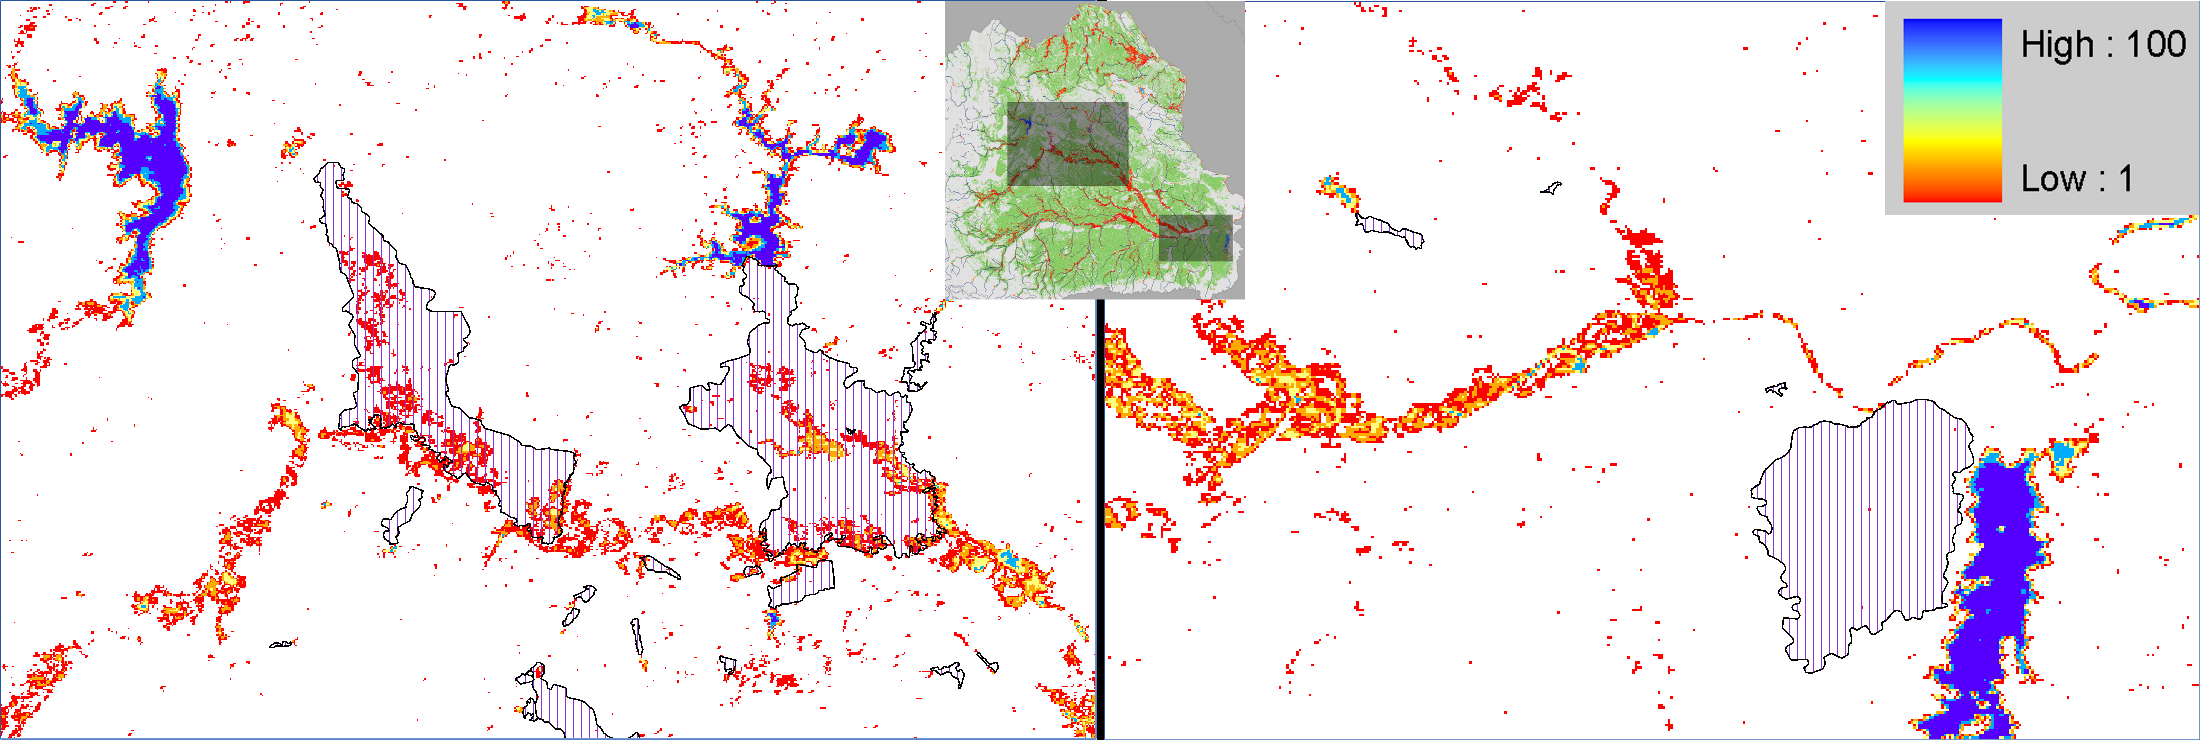
\includegraphics[width=11cm]{NETH_ASO_FREQ_irrig_area_insert_big_legend}
\end{center}

\end{frame}

%%%%%%%%%%%%%%%%%%%%%%%%%%%%%%%%%%%%%%%%%%%%%%%%%%%%%%%%%%%%%%%%%%%%
\begin{frame}[fragile]{Rice submergence occurence for large areas}

\begin{center}
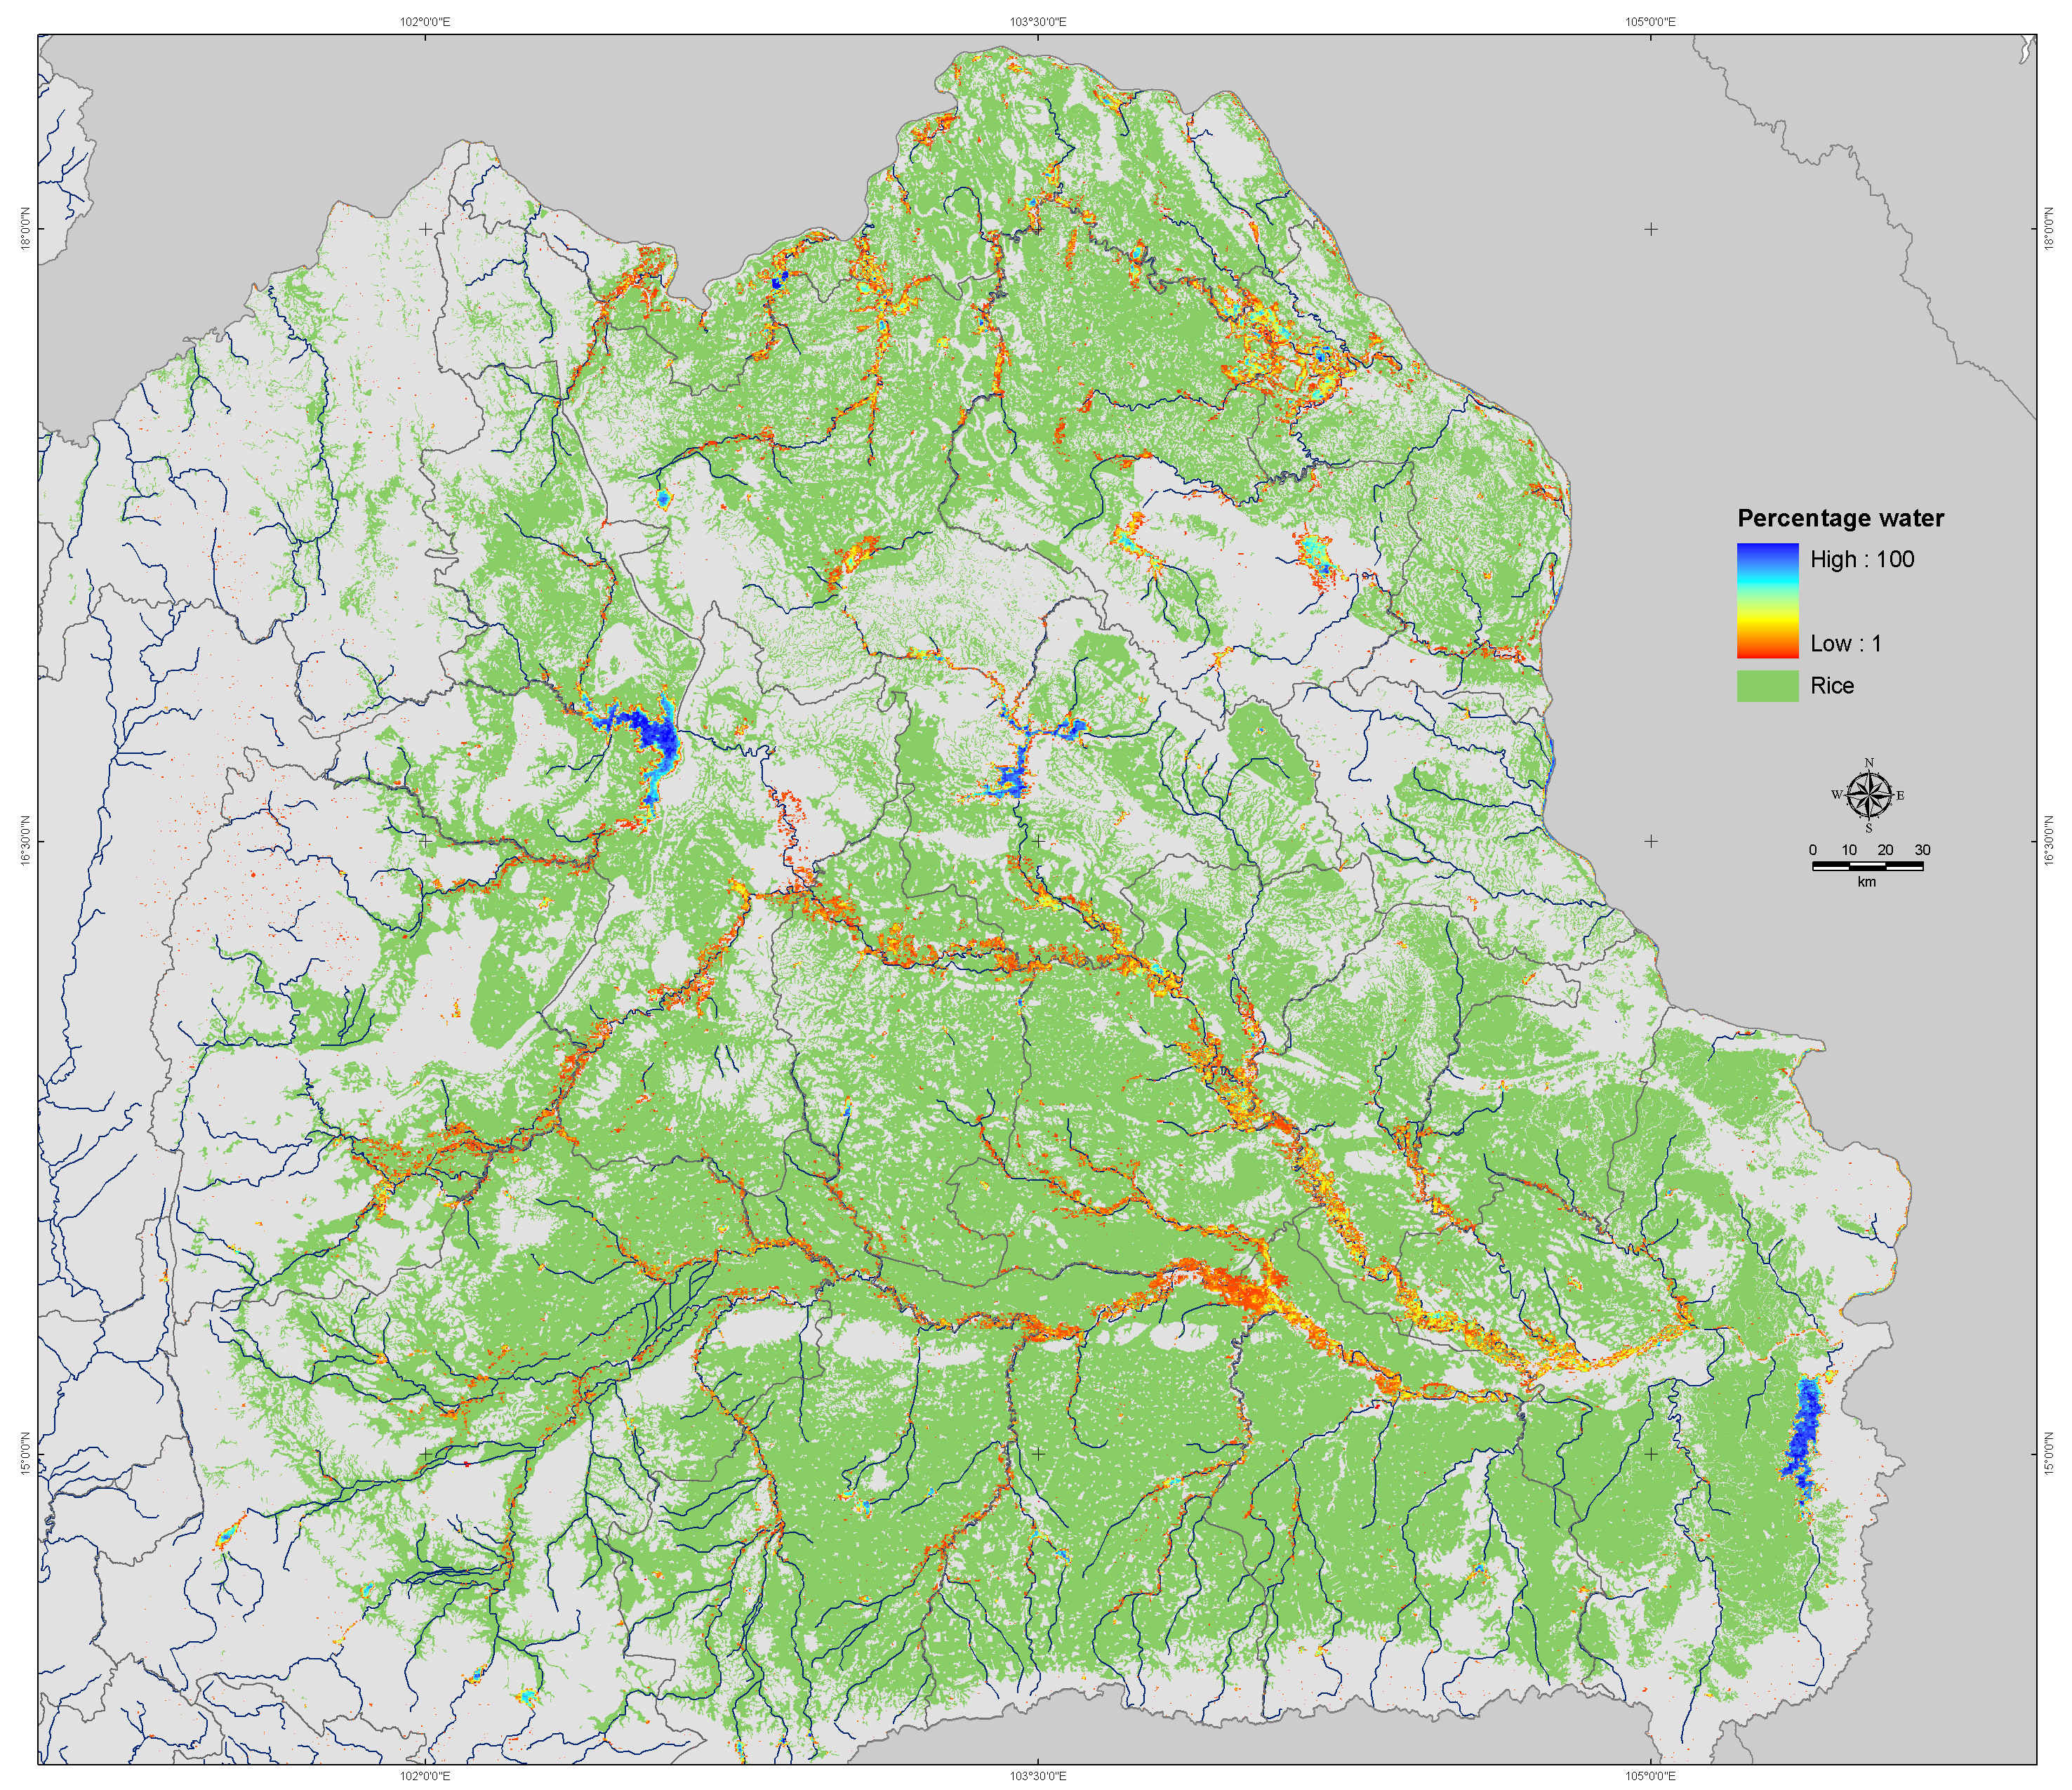
\includegraphics[width=8cm]{NETHA_Freq_Sep}
\end{center}

\end{frame}

%%%%%%%%%%%%%%%%%%%%%%%%%%%%%%%%%%%%%%%%%%%%%%%%%%%%%%%%%%%%%%%%%%%%
\begin{frame}[fragile]{Rice Irrigated Area Risk}

\begin{center}
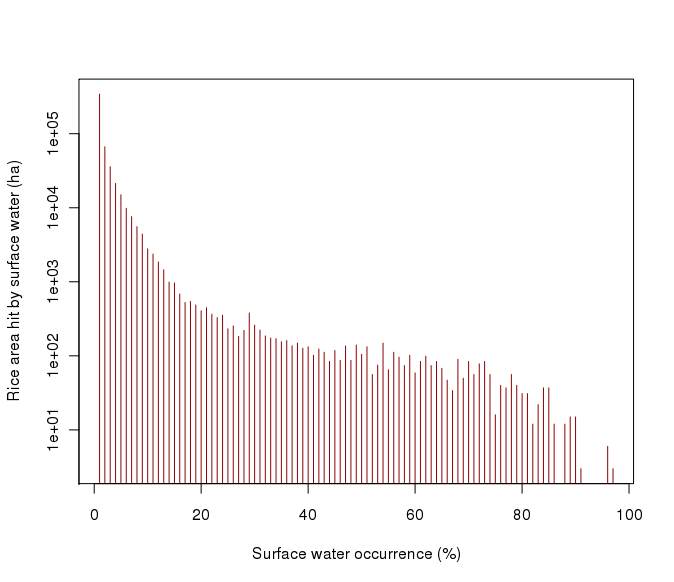
\includegraphics[width=8cm]{NETH_histogram_rice}
\end{center}

\end{frame}

%%%%%%%%%%%%%%%%%%%%%%%%%%%%%%%%%%%%%%%%%%%%%%%%%%%%%%%%%%%%%%%%%%%%
\begin{frame}[fragile]{Rice Temporal Submergence Risk (Event-based)}

\begin{center}
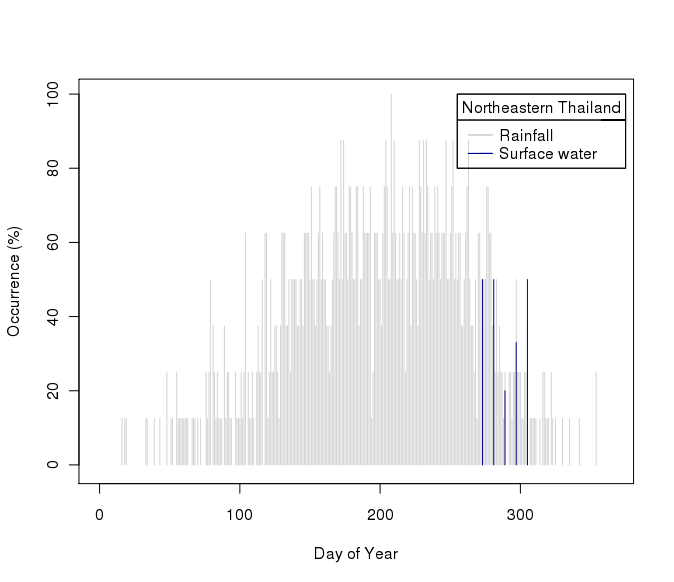
\includegraphics[width=8cm]{NETH_daily}
\end{center}

\end{frame}


\section{Water Stress}
%%%%%%%%%%%%%%%%%%%%%%%%%%%%%%%%%%%%%%%%%%%%%%%%%%%%%%%%%%%%%%%%%%%%
\begin{frame}[fragile]{Yield, Water \& Land Productivity}

\begin{flushleft}
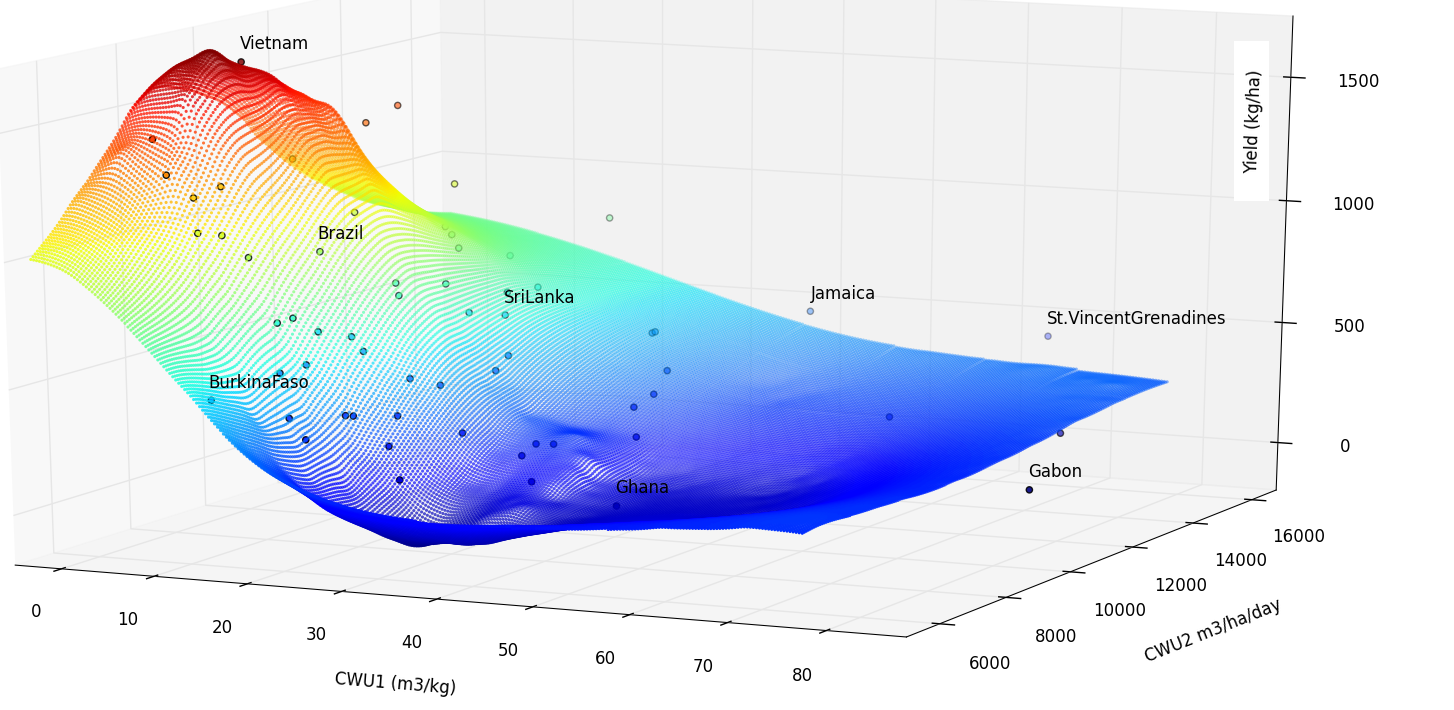
\includegraphics[width=13cm]{3d}
\end{flushleft}

\end{frame}

%%%%%%%%%%%%%%%%%%%%%%%%%%%%%%%%%%%%%%%%%%%%%%%%%%%%%%%%%%%%%%%%%%%%
\begin{frame}[fragile]{Environmental Water Stress}

\begin{flushleft}
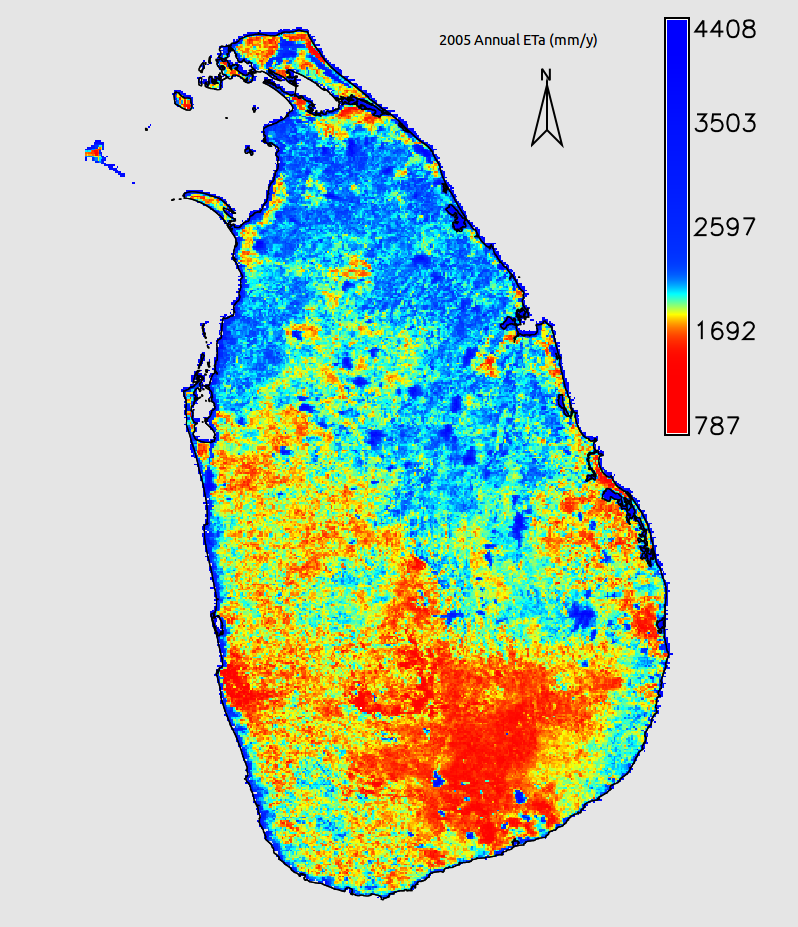
\includegraphics[width=5.5cm]{slet2005} 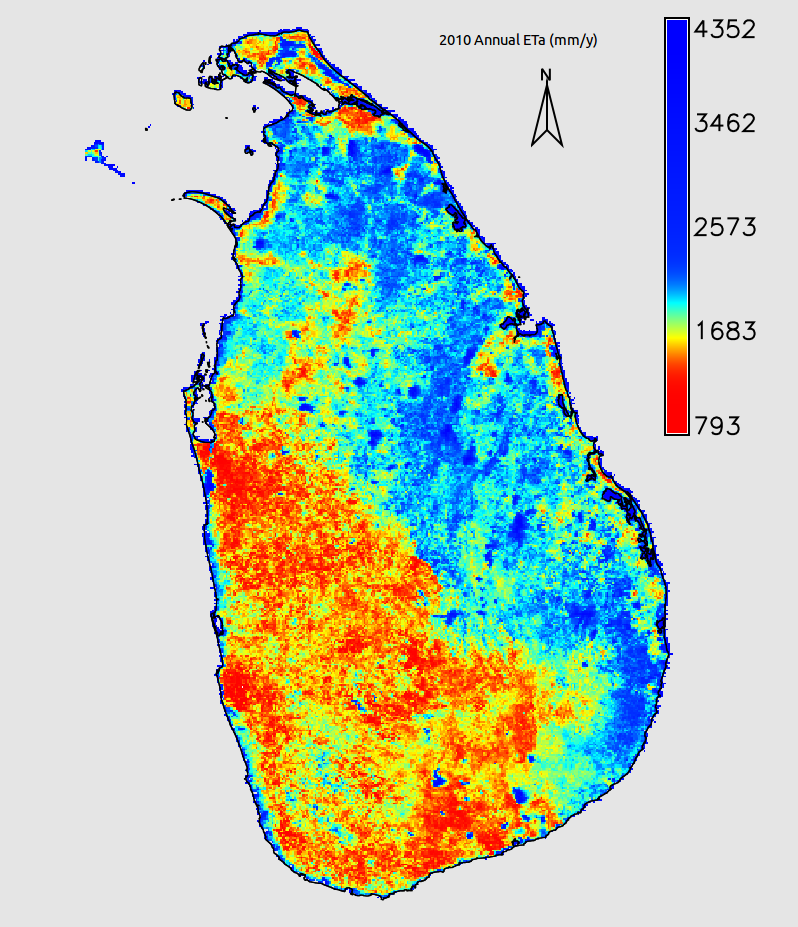
\includegraphics[width=5.5cm]{slet2010} 
\end{flushleft}

\end{frame}



\section{Conclusions}
%%%%%%%%%%%%%%%%%%%%%%%%%%%%%%%%%%%%%%%%%%%%%%%%%%%%%%%%%%%%%%%%%%%%
\begin{frame}[fragile]{Conclusions}

 Public domain RS data is used for crop risk assessment
\begin{enumerate}
 \item Space monitoring technology in space and time
 \item Landsat8 has 24 hours delivery, high resolution.
\end{enumerate}

\end{frame}

%%%%%%%%%%%%%%%%%%%%%%%%%%%%%%%%%%%%%%%%%%%%%%%%%%%%%%%%%%%%%%%%%%%%
\begin{frame}[fragile]{Thank You}

\ \\
\ \\
\ \\
\ \\
\ \\
\ \\
\ 
\begin{flushright}
\begin{tabular}{r}

\includegraphics[width=2cm]{iwmi}\\
\end{tabular}
\end{flushright}

\end{frame}

\end{document}
